% !TEX TS-program = pdflatex
% !TEX encoding = UTF-8 Unicode

% - - - - - article template - - - - -

% This is a simple template for a LaTeX document using the "article" class.
% See "book", "report", "letter" for other types of document.

\documentclass[11pt]{article} % use larger type; default would be 10pt

\usepackage{ucs}
\usepackage[utf8x]{inputenc} % set input encoding (not needed with XeLaTeX)

\usepackage[german]{babel}

%%% Examples of Article customizations
% These packages are optional, depending whether you want the features they provide.
% See the LaTeX Companion or other references for full information.

%%% PAGE DIMENSIONS
\usepackage{geometry} % to change the page dimensions
\geometry{a4paper} % or letterpaper (US) or a5paper or....
\geometry{margin=3cm} % for example, change the margins to 2 inches all round
% \geometry{landscape} % set up the page for landscape
%   read geometry.pdf for detailed page layout information

\usepackage{graphicx} % support the \includegraphics command and options
\usepackage{epstopdf}

% \usepackage[parfill]{parskip} % Activate to begin paragraphs with an empty line rather than an indent

%%% PACKAGES
\usepackage{booktabs} % for much better looking tables
\usepackage{array} % for better arrays (eg matrices) in maths
\usepackage{paralist} % very flexible & customisable lists (eg. enumerate/itemize, etc.)
\usepackage{verbatim} % adds environment for commenting out blocks of text & for better verbatim
\usepackage{subfig} % make it possible to include more than one captioned figure/table in a single float
% These packages are all incorporated in the memoir class to one degree or another...

%%% HEADERS & FOOTERS
\usepackage{fancyhdr} % This should be set AFTER setting up the page geometry
\pagestyle{fancy} % options: empty , plain , fancy
\renewcommand{\headrulewidth}{0pt} % customise the layout...
\lhead{}\chead{}\rhead{}
\lfoot{}\cfoot{\thepage}\rfoot{}

%%% SECTION TITLE APPEARANCE
\usepackage{sectsty}
\allsectionsfont{\sffamily\mdseries\upshape} % (See the fntguide.pdf for font help)
% (This matches ConTeXt defaults)

%%% ToC (table of contents) APPEARANCE
\usepackage[nottoc]{tocbibind} % Put the bibliography in the ToC DOn't show lists of figures/tables: notlof,notlot
\usepackage[titles,subfigure]{tocloft} % Alter the style of the Table of Contents
\renewcommand{\cftsecfont}{\rmfamily\mdseries\upshape}
\renewcommand{\cftsecpagefont}{\rmfamily\mdseries\upshape} % No bold!

%%% END Article customizations



% - - - - - Anpassungen spezifisch für SSE - - - - -

\usepackage{struktex} %Struktogramme
\usepackage{todonotes} % \todo{} und \missingfigure{} und \listoftodos
\usepackage{listings} % Quellcode
\lstset{frame=single, numbers=left, numberstyle=\tiny, stepnumber=5, numbersep=5pt, basicstyle=\small, breaklines} % Default-Formatierung für Quellcode. language und tabsize noch gesetzt werden...
\usepackage{pdfpages} % externe PDF-Dokumente einbinden
\usepackage{changepage} %Seitenbreite ändern wenn nötig
\usepackage{float} \restylefloat{figure} % Möglichkeit, Bild genau hier positionieren mit \begin{figure}[H]
\usepackage{blindtext} % Lorem Ipsum-Ersatz



% - - - - - Anfang des Dokuments - - - - -
\begin{document}

% . . . . . Titelseite . . . . .
\begin{titlepage}
	\begin{center}
		\vspace*{1cm}
		
\includegraphics[width=0.3\textwidth]{tud_logo_blau_2133x626}\\
		\vspace{0.5cm}
		{\large Fakultät für Informatik}\\
		{\large Institut für Technische Informatik}\\
		\vspace{3cm}
		{\Large Beleg zum Komplexpraktikum Prozessorentwurf}\\
		\vspace{1cm}
		{\huge Entwurf eines einfachen Mikroprozessors mit dreistufiger Pipeline}\\
		\vspace{1cm}
		{\Large Kandetzki Valentin}\\
		\vspace{0.5cm}
		Matrikelnummer: 3755109\\
		Studiengang: Informationssystemtechnik\\
		Studienjahrgang: 2011\\
		\vspace{1cm}
		{\Large Kemnitz Alexander}\\
		\vspace{0.5cm}
		Matrikelnummer: 3755118\\
		Studiengang: Informationssystemtechnik\\
		Studienjahrgang: 2011\\
		\vfill
		
		\large Dresden, \today\\
		\vspace{2cm}
		\large Verantwortlicher Hochschullehrer: Prof. Dr.-Ing. habil. Rainer G. Spallek\\
		\large Verantwortlicher Betreuer: Dr.-Ing. Martin Zabel\\
		\vspace*{1cm}
\end{center}
\end{titlepage}

% . . . . . Inhaltsverzeichnis . . . . .
\tableofcontents
\newpage


% . . . . . Einleitung . . . . .
\section{Aufgabenstellung}
Die Aufgabe bestand darin, einen einfachen Mikroprozessor mit reduzierten MIPS-Befehlssatz zu entwickeln.
Dabei war der Prozessor mit Steuerwerk, Datenpfad und 3-stufiger Pipeline sowie der Datenbus mit Wishboneprotokoll in VHDL zu implementieren. Die Komponenten I/O-Controller für UART, ALU sowie Programm- und Datenspeicher waren gegeben.
Ziel der Arbeit sollte es sein, ein "Hello World" Programm mit Hilfe des Mikroprozessors auf einem FPGA ausführen zu lassen.




% . . . . . Todo-Liste - vor dem Drucken auskommentieren :-) . . . . .
\vspace{2cm}

\subsection{Abarbeitungsreihenfolge}
\begin{description}
\item[1.] Blockdiagramm des Prozessors mit den einzelnen Komponenten und Verbindung zwischen ihnen

\item[2.] Implementierung der einzelnen Komponenten in VHDL, testen der Einzelkomponenten

\item[3.] Zusammenschalten der Komponenten im Topmodul

\item[4.] Test, Simulation und Debugging des Mikroprozessors

\item[5.] Portieren des Entwurfes auf ein FPGA und ausführen des Hello World Programms
\end{description}


\newpage


% . . . . . Hauptteil . . . . .
\section{Entwurf}
%Meine Empfehlung: Hauptteil aufteilen in Algorithmus - Realisierung - Simulation

Zu Beginn entwickelten wir mit Hilfe des Buchs "Patterson; Henessy: 
Rechnerorganisation und -entwurf" eine Grafische Darstellung der Komponenten des Prozessors. Um diese einfach bearbeiten zu können verwendeten wir das Programm Yed. (Endgültige version siehe Abbildung 1)
\vspace*{1cm}

{\Large Die wichtigsten Bestandteile sind:}\\


\subsection{PC (ProgrammCounter)}
Einfaches Register, das die Adresse des Aktuellen Befehls anzeigt. Dadurch, dass der Befehl getaktet aus dem Ram geladen wird, muss man i.A. den nächsten PC, den NPC, dafür verwenden. Ausnahme sind Programmstart und angehaltene Pipeline.

\subsection{J-adr-calc}
Hier wird abhängig vom Sprung typ Die Adresse berechnet. Es gibt drei Typen, die mittels j\_dst\_control unterschieden werden. 
\\Jump Target: Zieladresse = PC + Target&&"00". 
\\Jump immediate: Zieladresse = immediate 
\\(mit Übernahme der Obersten Bits der alten Adresse). 
\\Jump register: Zieladresse= Registerinhalt.

\subsection{Steuerung}
In der Steuerung wird für jeden Befehl entschieden, welche anderen Komponenten des MIPS verwendet werden und wie sie miteinander verbunden sind. 

 \begin{description}
 \item[J\_dst\_controll] Bestimmt die Art auf die die Zieladresse eines Sprungs berechnet wird. (J-Typ, R-Typ, I-Typ)
 \item[MemRead] signalisiert eine Load-Operation
 \item[MemWrite] signalisiert eine Write-Operation
 \item[MemToReg] gibt an Welches Ergebnis in ein Register gespeichert wird: Normales ALU-Ergebnis, Daten aus dem RAM oder die Rücksprung-Adresse bei JALR
 \item[AluOp] legt die Operation der ALU fest
 \item[RegWr] Signalisiert, ob ein Ergebnis in ein Register geschrieben werden soll. 
 \item[AluSrc] bestimmt, ob die Alu 2 Registerinhalte oder ein Register (rs) mit dem Immediate verrechnet wird.
 \item[jumpOp] Unterscheidet zwischen den Bedingungen für einen Sprung. Es gibt auch jeweils einen Wert für kein Sprung und unbedingter Sprung.
 \item[ShiftSrc] dient bei Shift-Operationen zur Unterscheidung zwischen Registerwert und 'Immediate' 
 \item[Branch] Kündigt einen Potientiellen Sprung an, damit der übernächste Befehl eventuell nicht ausgeführt wird.
 \item[RegDst] Entscheidet ob auf rt oder rd zurückgeschrieben wird
 \item[link] Legt fest, dass bei JALR  die Rücksprungadresse auf R31 (ra) gesichert wird.
 \end{description}
 Des weiteren gibt es noch die Steuersignal j (in comparator berechnet), das festlegt, ob der Nächste Befehl Sequentiell berechnet wird oder ein Sprungziel ist und pipeline\_Enable (im Speicherinterface berechnet), das die Pipeline bei LOAD/STORE-Befehlen stoppt.

\subsection{Registers}
Enthält die Register 31 Register, wobei R0 fest mit 0 verdrahtet ist. Es können im gleichen Takt 2 Register ausgelesen und 1 Register beschrieben werden, wobei das Lesen in ID-Stufe und das Schreiben in der EX-Stufe eines Befehls ausgeführt wird. Daraus ergibt sich, dass wenn ein Befehl das Ergebnis des letzten Befehls benötigt (read und write Addresse gleich sind), das Ergebnis direkt weitergegeben wird, da das Ergebnis ja erst einen Takt zu spät im Register stehen würde.

\subsection{sgn-extend}
Dient lediglich zur vorzeichenbehafteten Erweiterung des Immediates auf 32, weil der Immediate 16 Bit groß ist, während die Alu mit 32 Bit rechnet.

\subsection{Comparator}
Überprüft für bedingte Sprünge, ob die Bedingungen erfüllt sind. Es gibt die Bedingung on Equal, on not Equal, wo Data1 mit Data2 verglichen wird  sowie on greater than, less then, reager equal, less equal zero, wo Data1 mit 0 verglichen wird.

\subsection{Memory Interface}
Verbindet den Prozessor mit RAM und UART. Dabei ist unser Interface Schnittstelle zwischen LOAD/STORE-befehlen und Wishbone-Protokoll. Dieses Interface beinhaltet den Master des Protokolls. Weil die Datenübertragung mehrere Takte benötigt, wird der Pipeline hier solange angehalten bis die Übertragung abgeschlossen ist. Im Fall des RAMs ist das eine feste Zeitspanne in Fall der UART variable Zeit, die durch das Wishboneprotokoll und die angehaltene Pipeline allerdings keinen Einfluss auf den Programmverlauf hat. 
Im nachfolgenden Bild ist der Zustandsgraf der FSM beigelegt.

\begin{figure}[h!]
\centering
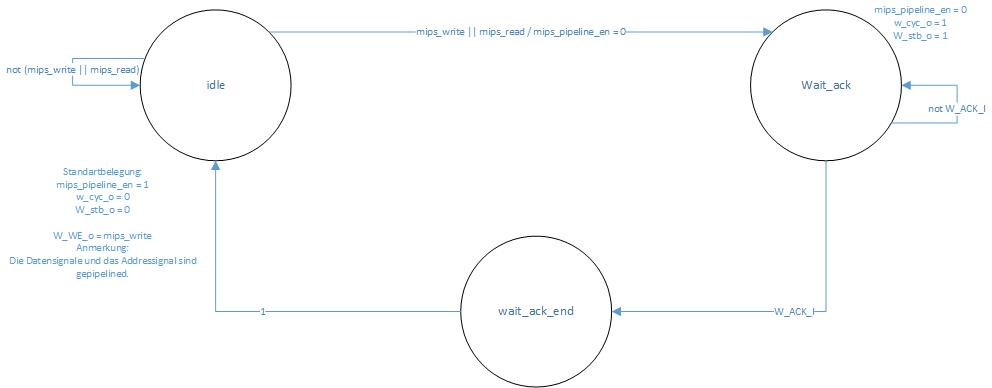
\includegraphics[width=1\textwidth]{FSM_WBmaster}
\caption{FSM\_WB\_Master}
\end{figure}

\subsection{Pipelineregister IF-ID}
erstes Pipelineregister

\subsection{Pipelineregister ID-EX}
zweites Pipelineregister

\subsection{ALU}
gegeben, Rechenwerk des Prozessors

\subsection{Operationstypen:}
 - Rechenbefehl\
    Signalbelegungen: Operation ALU op. Branch, MemRead, MemWrite, link, .. 0. MemToReg 0. Shiftsource nur bei Shift operation abhängig Register/'Immediate'.\\
    RegDst und AluSrc abhäning von Imm/2 Register
  \\ - Immediate 
  \\ - 2 Register
 \\- Load/Store
 \\- Sprungbefehl
  \\ Sprungbefehle führen in einer 3-Stufigen Pipeline bereits zu einem Harzad. Deswegen wird der Befehl 2 nach dem Sprungbefehl durch eine NOP ersetzt (auch wenn der Sprung am Ende nciht ausgeführt wird). Dafür ist das Signal Branch zuständigk, das einen Potentiellen Sprung markiert.
    \\Unterteilung in Bedingung (in comporator geprüft) zuständiges \\Signal: jumpOp
  \\ (-kein Sprung) 
   \\- unbedingt
   \\- bedingt
     \\- Vergleich zweier Registerinhalte
       \\- auf Gleichheit
       \\- auf Ungleichheit
     \\- Vergleich eines Registerinhalts mit 0
       \\- größer
       \\- kleiner
       \\- größer oder gleich
       \\- kleiner oder gleich
    \\und Typ der Zieladresse (J-adr-calc geprüft) : zuständiges \\Signal J_dst_control
 \\  - Jump (target)
   \\- Jump Register
   \\- Jump Immediate
\end{description}


\begin{figure}
\centering
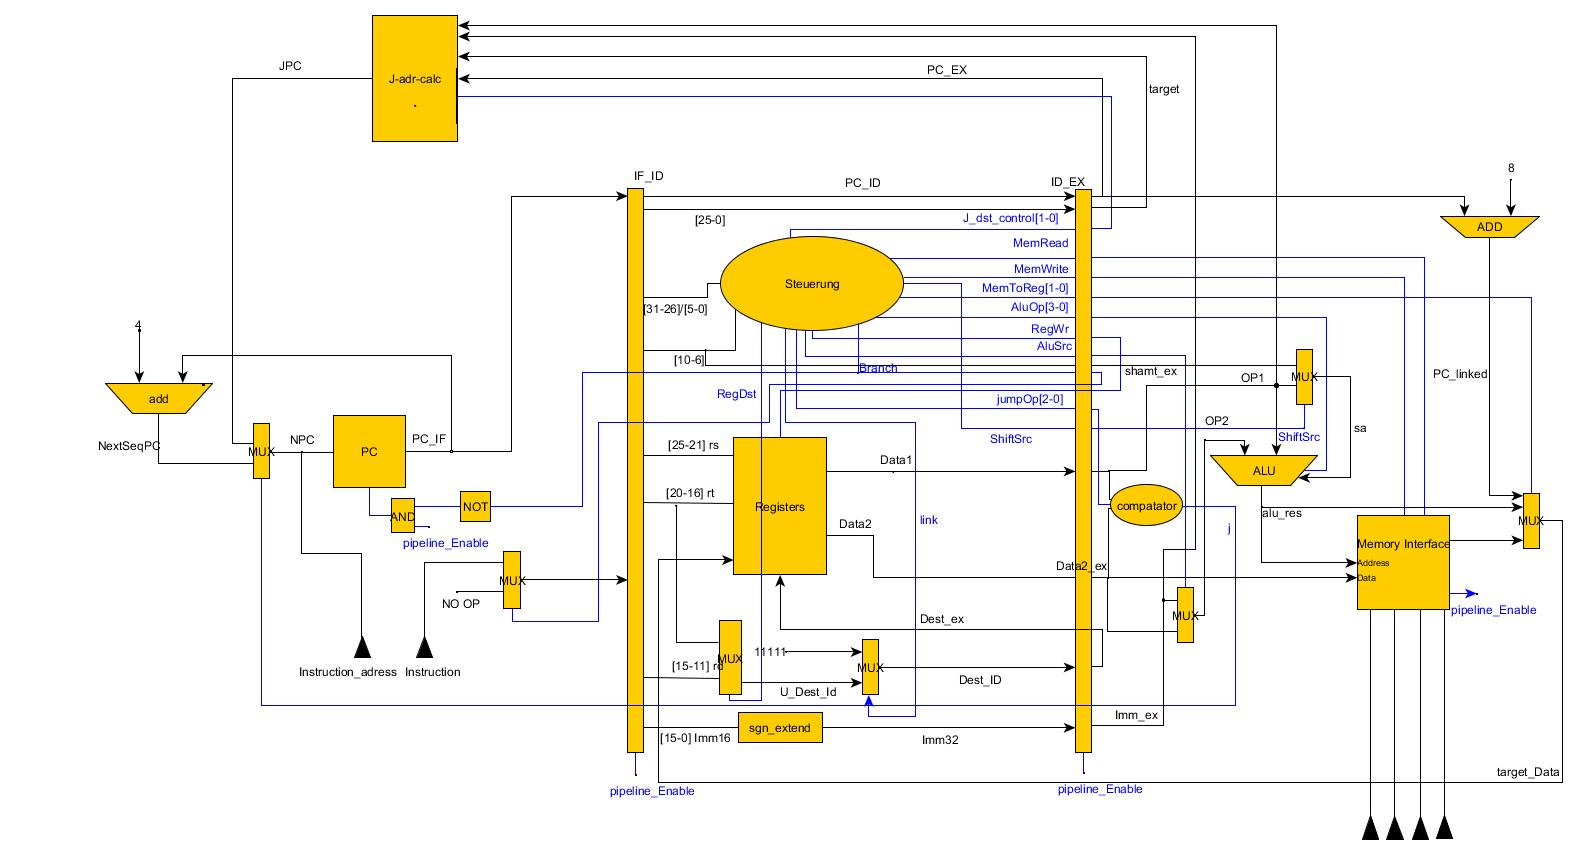
\includegraphics[width=1.4\textwidth, angle=90]{Prozessorentwurf_Komponenten_jumps}
\caption{Komponenten}
\end{figure}

\newpage
\section{Test}
\subsection{Comparator}
Es gibt je 4 Testfälle zu den Operation branch on equal, branch on not equal, no jump.
Bei branch on equal / branch on not equal werden im ersten Fall zwei gleiche Zahlen miteinander verglichen (zwei Nullen). Im zweiten Fall zwei ungleiche Zahlen und im dritten zwei gleiche Zahlen ungleich null. Das Ergebnis soll bei branch on not equal im Fall eins „0“ sein, im Fall zwei „1“ und im Fall drei „0“. Die Ergebnisse zu Branch on equal sind entsprechend invers.
Im Testfall no Jump werden Operationen getestet, in denen kein Sprung ausgeführt werden soll.
\subsection{J\_adr\_calc}
Im Test des J\_adr\_calc werden verschiedene Werte („00“, „01“, „10“) für J\_dst\_control verwendet und geprüft, ob die Richtige Sprungadresse berechnet wurde.
Registers
\subsection{Steuerung}
In der Testbench der Steuerung werden die Ergebnisse der Ausgangssignale für die Einzelnen Befehle (Operationen) getestet. Bei der Operation“000000“ wird hierbei „funct“ genauer betrachtet.\\
funct <= "000000"  = SLL\\
funct <= "000010" = SLR\\
funct <= "000011" = SRA\\
funct <= "000100" = SLLV\\
funct <= "000110" = SLRV\\
funct <= "000111" = SRAV\\
funct <= "100000" = ADD\\
funct <= "100001" = ADDU\\
funct <= "100010" = SUB\\
funct <= "100011" = SUBU\\
funct <= "100100" = AND\\
funct <= "100101" = OR\\
funct <= "100110" = XOR\\
funct <= "100111" = NOR\\
funct <= "101010" = SLT\\
funct <= "101011" = SLTU\\
funct <= "001000" = JR\\
funct <= "001001" = JALR\\
\newpage\\
operation <= "000010" = J\\
operation <= "000011" = JAL\\
operation <= "000100" = BEQ\\
operation <= "000101" = BNE\\
operation <= "001000" = ADDI\\
operation <= "001001" = ADDIU\\
operation <= "001010" = SLTI\\
operation <= "001011" = SLTIU\\
operation <= "001100" = ANDI\\
operation <= "001101" = ORI\\
operation <= "001110" = XORI\\
operation <= "001111" = LUI\\
operation <= "100011" = LW\\
operation <= "101011" = SW\\

Die Erwarteten Ausgangssignale können dem Quellcode entnommen werden.
\subsection{Wishbone\_Master}
Für den Wishbone Master werden drei Testfälle unterschieden. (Store Word, Load Word und read and write).
Dabei soll bei Store Word auf denRam geschrieben werden und bei Load Word von dort Geladen werden. Bei read and write tritt ein Fehler auf.
\subsection{mips\_top}
Hier wir die Zusammenschaltung der einzelnen Komponenten getestet.
Dabei werde direkte Assemblerbefehle wie Add, Sub, Or, Jump getestet und geschaut ob die Registerinhalte dem richtigen Ergebnis entsprechen.
\subsection{Megatop}
Hier werden ebenfalls Assemblerbefehle getestet. Da der bootram hier mit enthalten ist können auch die Load- und Stoarebefehle getestet werden.

\begin{figure}[h!]
\centering
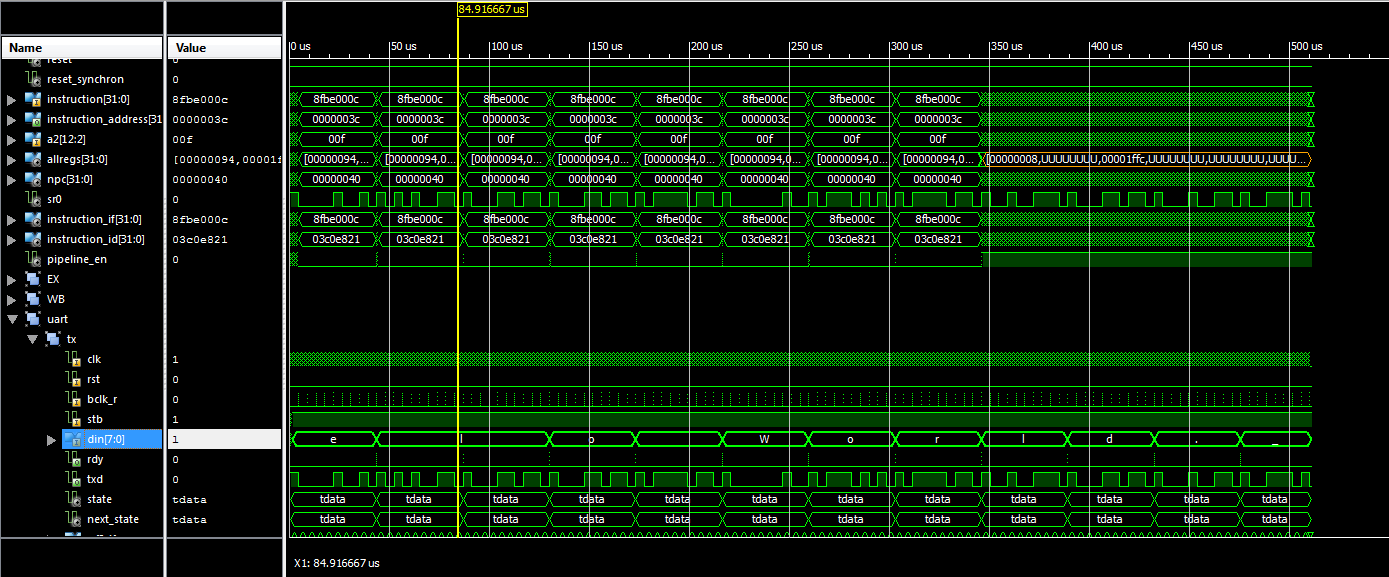
\includegraphics[width=1\textwidth]{Hello World Waveforms.png}
\caption{Hello World Ausgabe}
\end{figure}

\begin{figure}[h!]
\centering
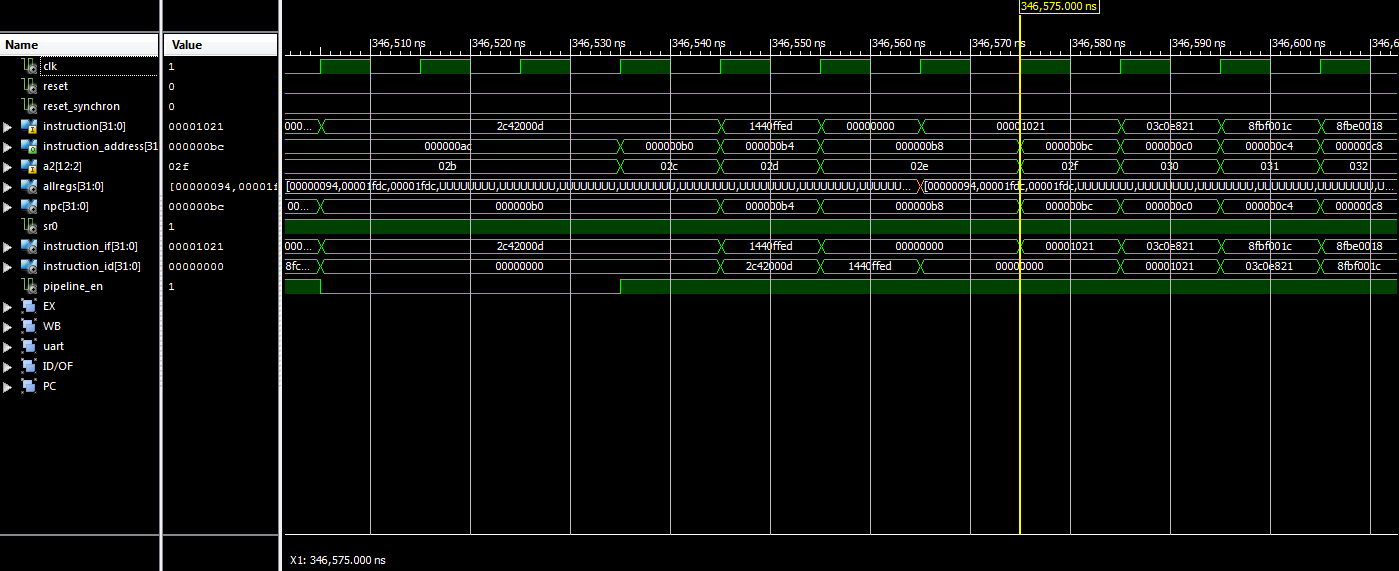
\includegraphics[width=1\textwidth]{Branch condition false Waveforms.png}
\caption{Branch condition false Waveforms}
\end{figure}

\begin{figure}[h!]
\centering
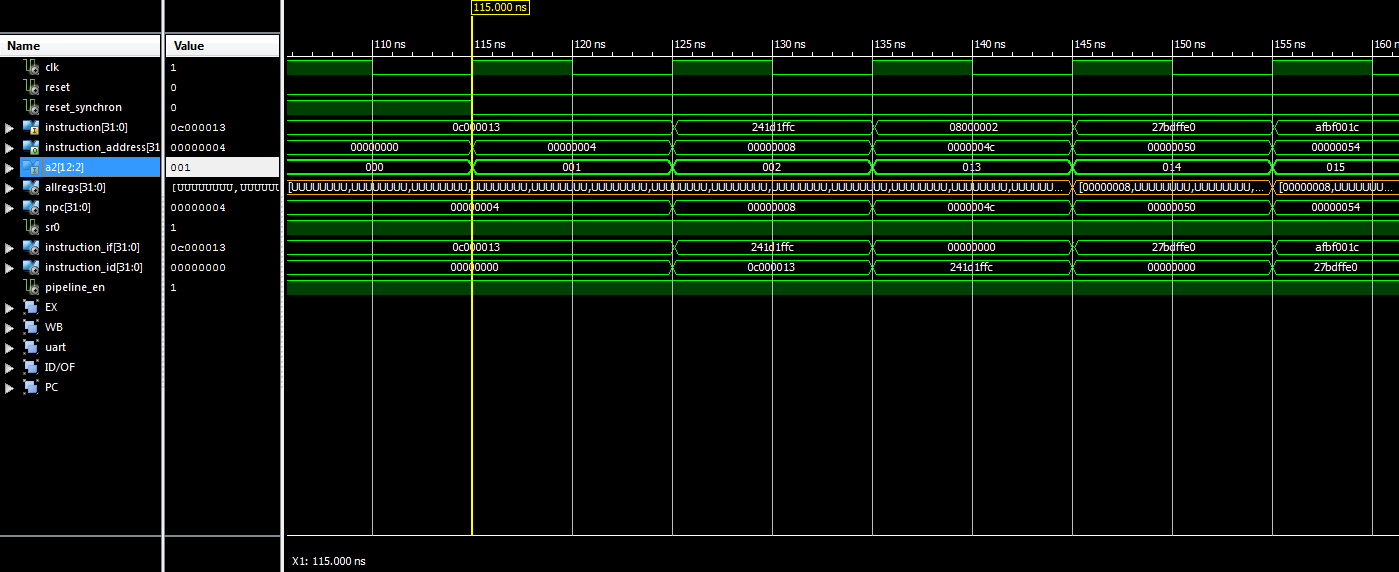
\includegraphics[width=1\textwidth]{Start Waveforms.png}
\caption{Start Waveforms}
\end{figure}

\begin{figure}[h!]
\centering
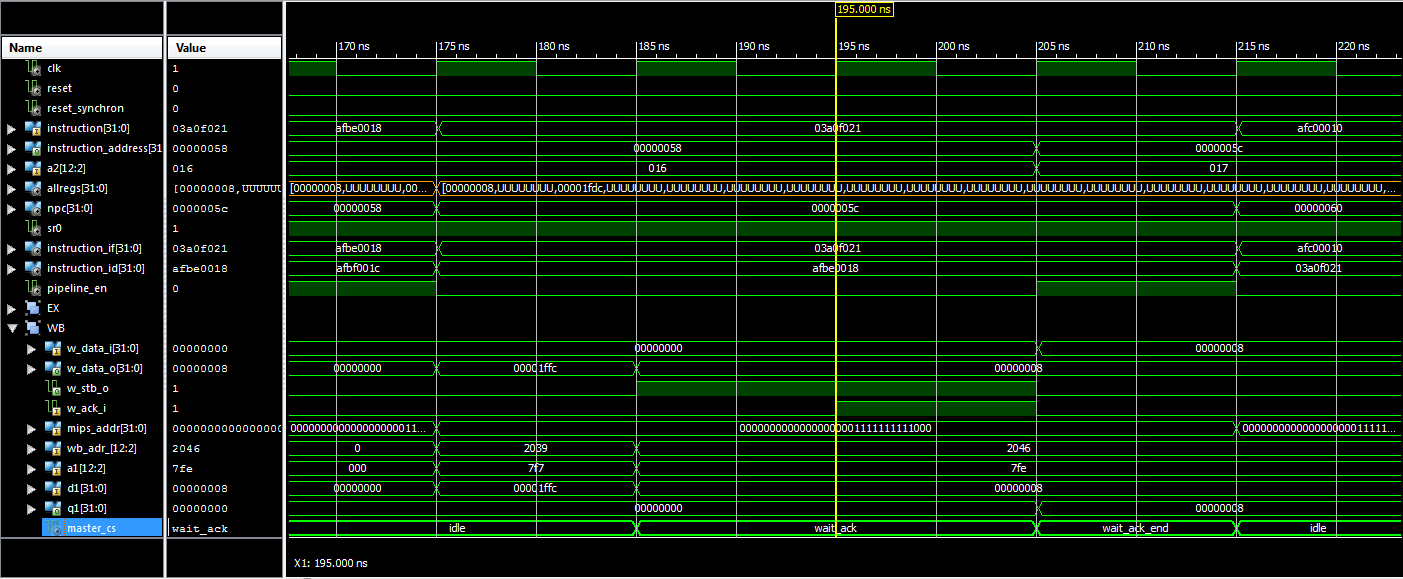
\includegraphics[width=1\textwidth]{wishbone handshake waveforms.png}
\caption{wishbone handshake waveforms}
\end{figure}

\begin{figure}[h!]
\centering
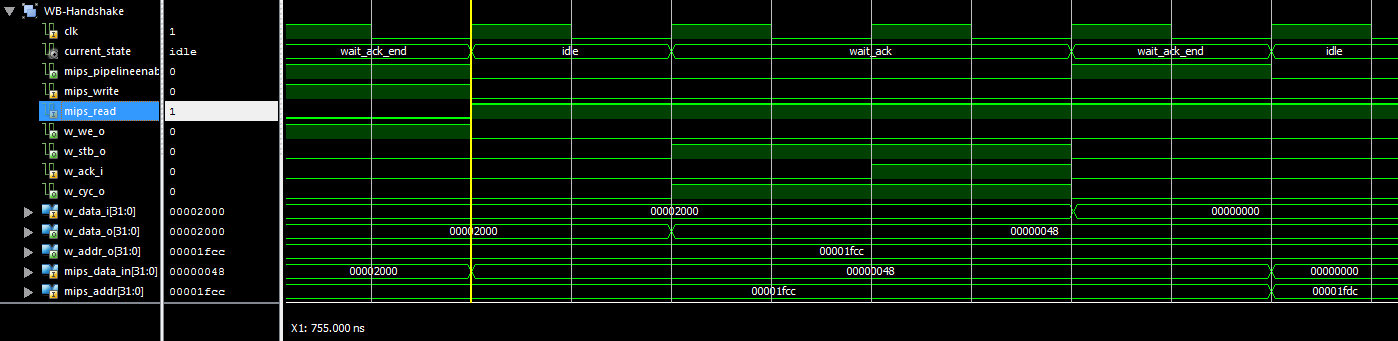
\includegraphics[width=1\textwidth]{wishbone handshake LOAD waveforms.png}
\caption{wishbone handshake LOAD waveforms}
\end{figure}

\begin{figure}[h!]
\centering
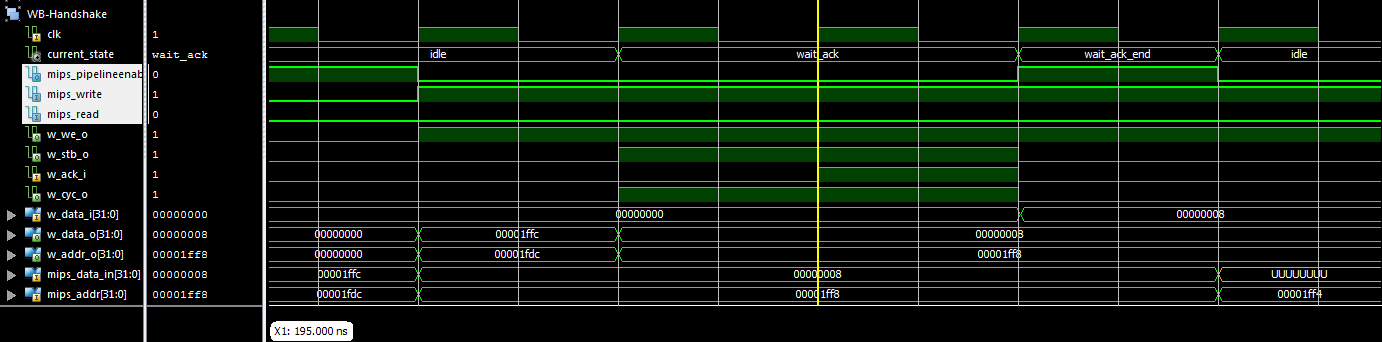
\includegraphics[width=1\textwidth]{wishbone handshake STORE waveforms.png}
\caption{wishbone handshake STORE waveforms}
\end{figure}


\newpage
% . . . . . Verzeichnisse . . . .
\newpage
\listoffigures
\vfill
\end{thebibliography}
\vfill
\end{document}
